% Options for packages loaded elsewhere
\PassOptionsToPackage{unicode}{hyperref}
\PassOptionsToPackage{hyphens}{url}
%
\documentclass[
]{article}
\usepackage{amsmath,amssymb}
\usepackage{lmodern}
\usepackage{iftex}
\ifPDFTeX
  \usepackage[T1]{fontenc}
  \usepackage[utf8]{inputenc}
  \usepackage{textcomp} % provide euro and other symbols
\else % if luatex or xetex
  \usepackage{unicode-math}
  \defaultfontfeatures{Scale=MatchLowercase}
  \defaultfontfeatures[\rmfamily]{Ligatures=TeX,Scale=1}
\fi
% Use upquote if available, for straight quotes in verbatim environments
\IfFileExists{upquote.sty}{\usepackage{upquote}}{}
\IfFileExists{microtype.sty}{% use microtype if available
  \usepackage[]{microtype}
  \UseMicrotypeSet[protrusion]{basicmath} % disable protrusion for tt fonts
}{}
\makeatletter
\@ifundefined{KOMAClassName}{% if non-KOMA class
  \IfFileExists{parskip.sty}{%
    \usepackage{parskip}
  }{% else
    \setlength{\parindent}{0pt}
    \setlength{\parskip}{6pt plus 2pt minus 1pt}}
}{% if KOMA class
  \KOMAoptions{parskip=half}}
\makeatother
\usepackage{xcolor}
\IfFileExists{xurl.sty}{\usepackage{xurl}}{} % add URL line breaks if available
\IfFileExists{bookmark.sty}{\usepackage{bookmark}}{\usepackage{hyperref}}
\hypersetup{
  pdftitle={People},
  hidelinks,
  pdfcreator={LaTeX via pandoc}}
\urlstyle{same} % disable monospaced font for URLs
\usepackage[margin=1in]{geometry}
\usepackage{graphicx}
\makeatletter
\def\maxwidth{\ifdim\Gin@nat@width>\linewidth\linewidth\else\Gin@nat@width\fi}
\def\maxheight{\ifdim\Gin@nat@height>\textheight\textheight\else\Gin@nat@height\fi}
\makeatother
% Scale images if necessary, so that they will not overflow the page
% margins by default, and it is still possible to overwrite the defaults
% using explicit options in \includegraphics[width, height, ...]{}
\setkeys{Gin}{width=\maxwidth,height=\maxheight,keepaspectratio}
% Set default figure placement to htbp
\makeatletter
\def\fps@figure{htbp}
\makeatother
\setlength{\emergencystretch}{3em} % prevent overfull lines
\providecommand{\tightlist}{%
  \setlength{\itemsep}{0pt}\setlength{\parskip}{0pt}}
\setcounter{secnumdepth}{-\maxdimen} % remove section numbering
\ifLuaTeX
  \usepackage{selnolig}  % disable illegal ligatures
\fi

\title{People}
\author{}
\date{\vspace{-2.5em}}

\begin{document}
\maketitle

Lab members listed alphabetically by last name. Last updated: June 2,
2022.

\begin{table}
\centering
\begin{tabular}[t]{>{\raggedright\arraybackslash}p{10em}|>{\raggedright\arraybackslash}p{15em}|>{\raggedright\arraybackslash}p{5em}|>{\raggedright\arraybackslash}p{20em}|>{\raggedright\arraybackslash}p{30em}}
\hline
 &  &  &  & \\
\hline
\textbf{Lauren Berry} & Master's Student & llberry@uark.edu & Lauren’s research interests include conservation management, population ecology, and avian ecology in response to our changing land use and climate. She is joining the Living Landscapes Lab to work on a project that will use data collected in and near three USFWS National Wildlife Refuges to create a mapping tool to quantify grassland bird and habitat core responses to grassland management. She has just finished her undergraduate work at Hendrix College, where she worked on a variety of projects including surveying urban wildlife in Central Arkansas, banding passerines at a Monitoring Avian Productivity and Survivorship station, and using Long Term Ecological Research Site data to evaluate insect population trends across North America. An Arkansas native, Lauren loves to backpack, cook, read, write, and spend time with her family in the southeastern part of the state. & \includegraphics{C:/Users/Caleb/Box/GitHub/RobertsLabWebsite2/images/ProfilePics/ProfilePic_LaurenBerry.jpg}\\
\hline
\textbf{Percy Marshall} & Master's Student & pmm005@uark.edu & Percy's research interests include behavioral ecology, landscape dynamics,and conservation ecology. They are specifically interested in the impacts of invasive waterfowl species on both natural ecosystems and private property. Percy's research will focus on cataloging distribution and abundance data on Egyptian Geese within Arkansas. They will be working towards understanding the risks that the waterfowl pose to human and ecological interests and helping better prepare for any management tactics that may be needed in the future. & 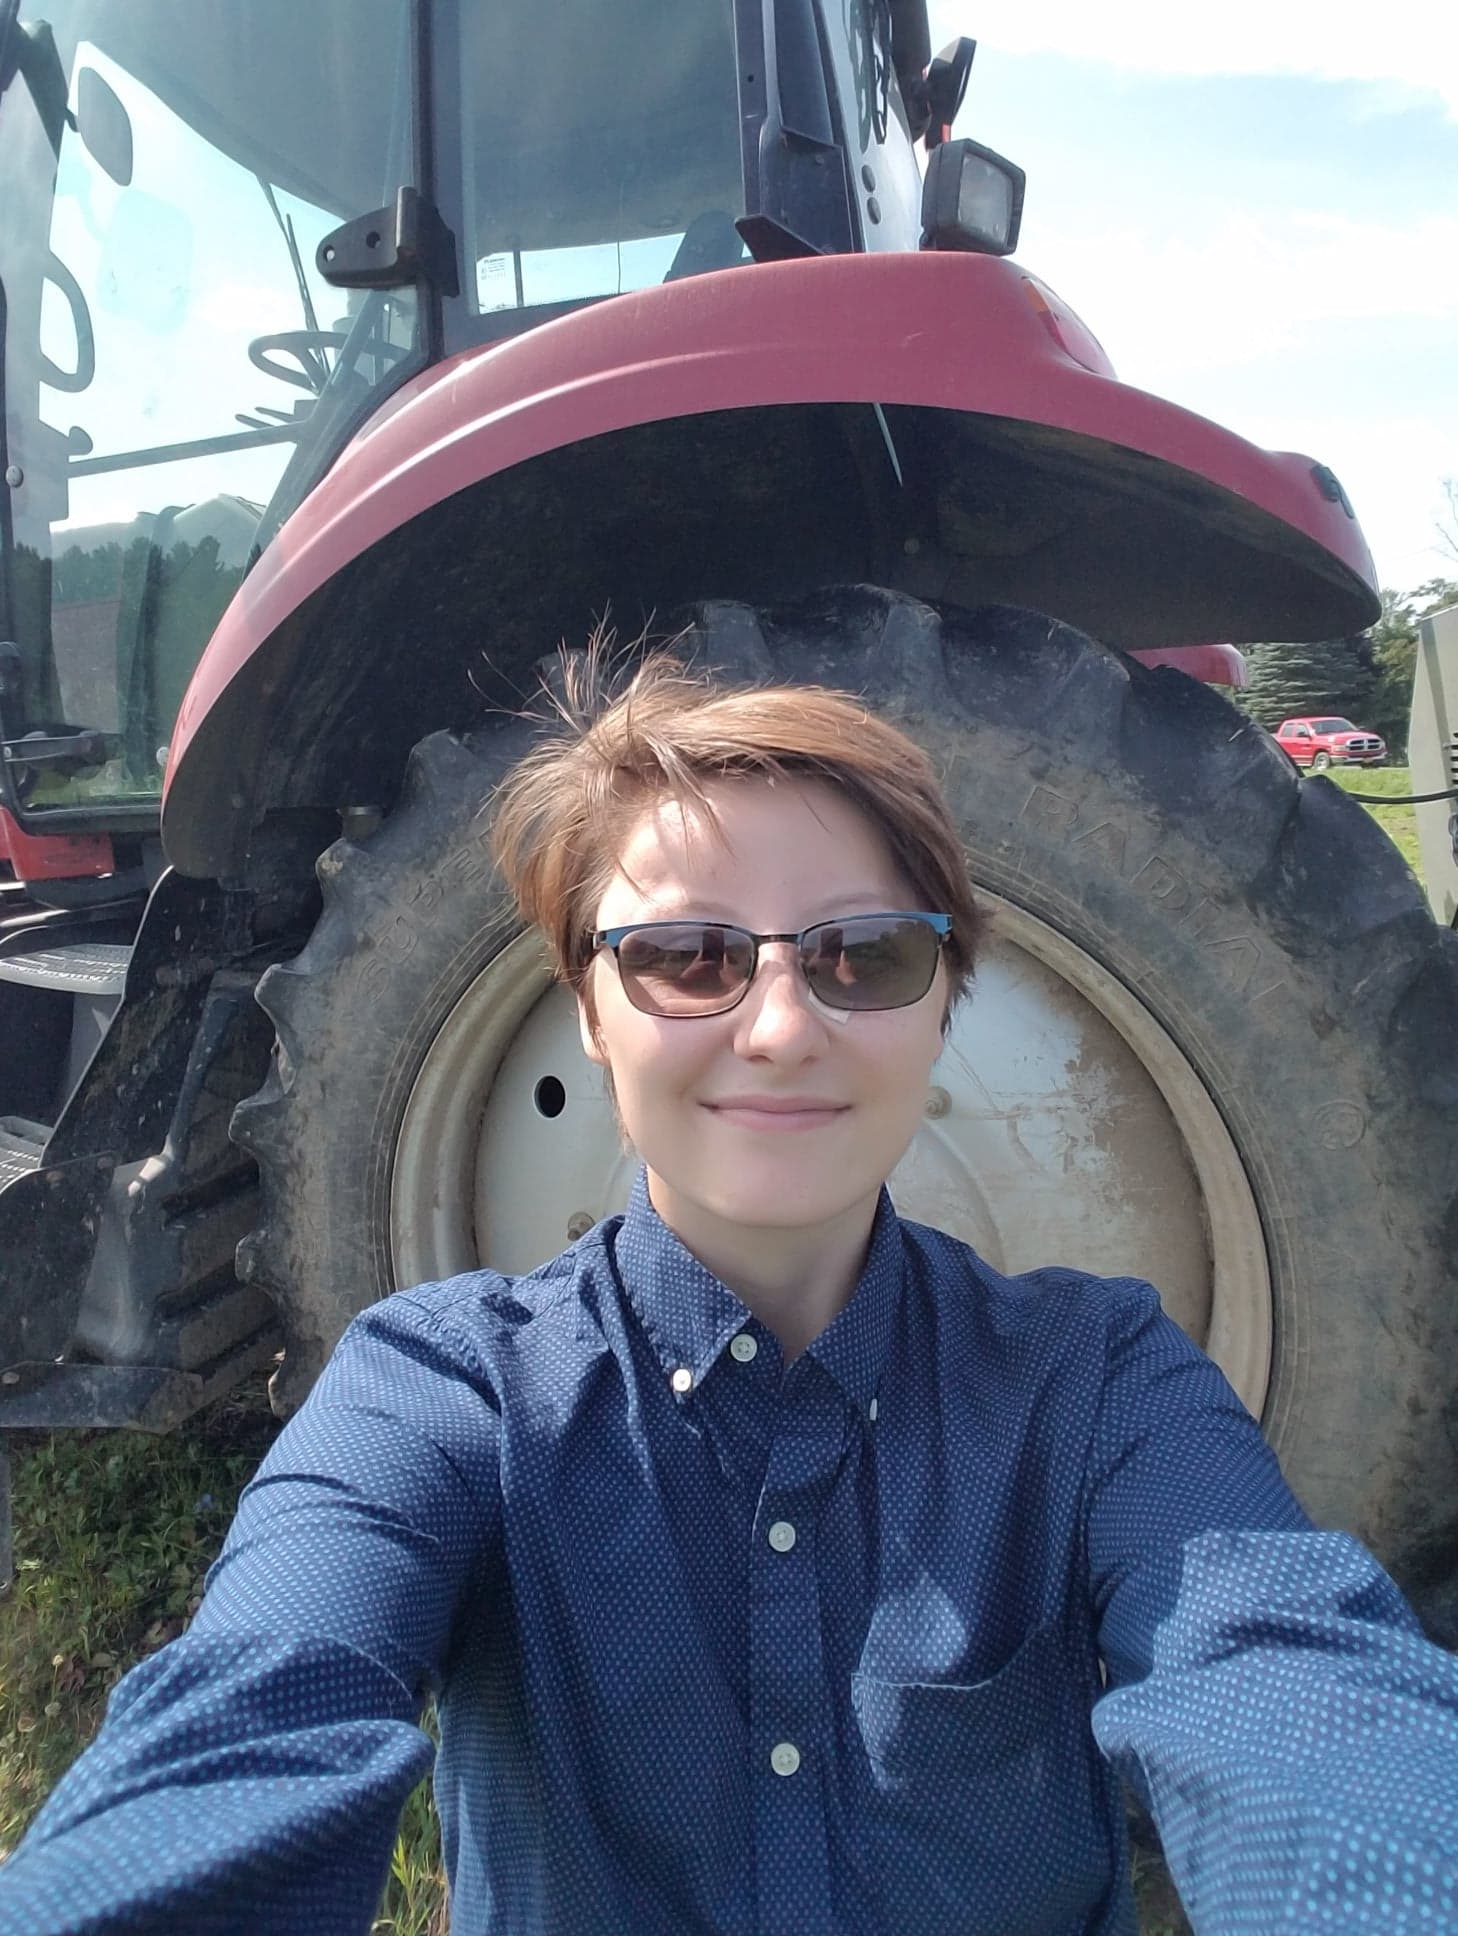
\includegraphics{C:/Users/Caleb/Box/GitHub/RobertsLabWebsite2/images/ProfilePics/ProfilePic_PercyMarshall.jpg}\\
\hline
\textbf{Caleb Roberts} & PI & cr065@uark.edu & Caleb is the leader of the Living Landscapes Lab. He works for the U.S. Geological Survey as an Assistant Unit Leader at the Arkansas Cooperative Fish \& Wildlife Research Unit. Caleb's research interests include ecological resilience, grasslands, landscape ecology, fire, birds, invasive species, plants, community ecology, agroecosystems, complexity theory, and rangelands. Caleb is from western Kentucky, and he enjoys writing, running, reading, cooking, gardening, board games, hiking, and hanging out with his wife, daughter, and cat. & 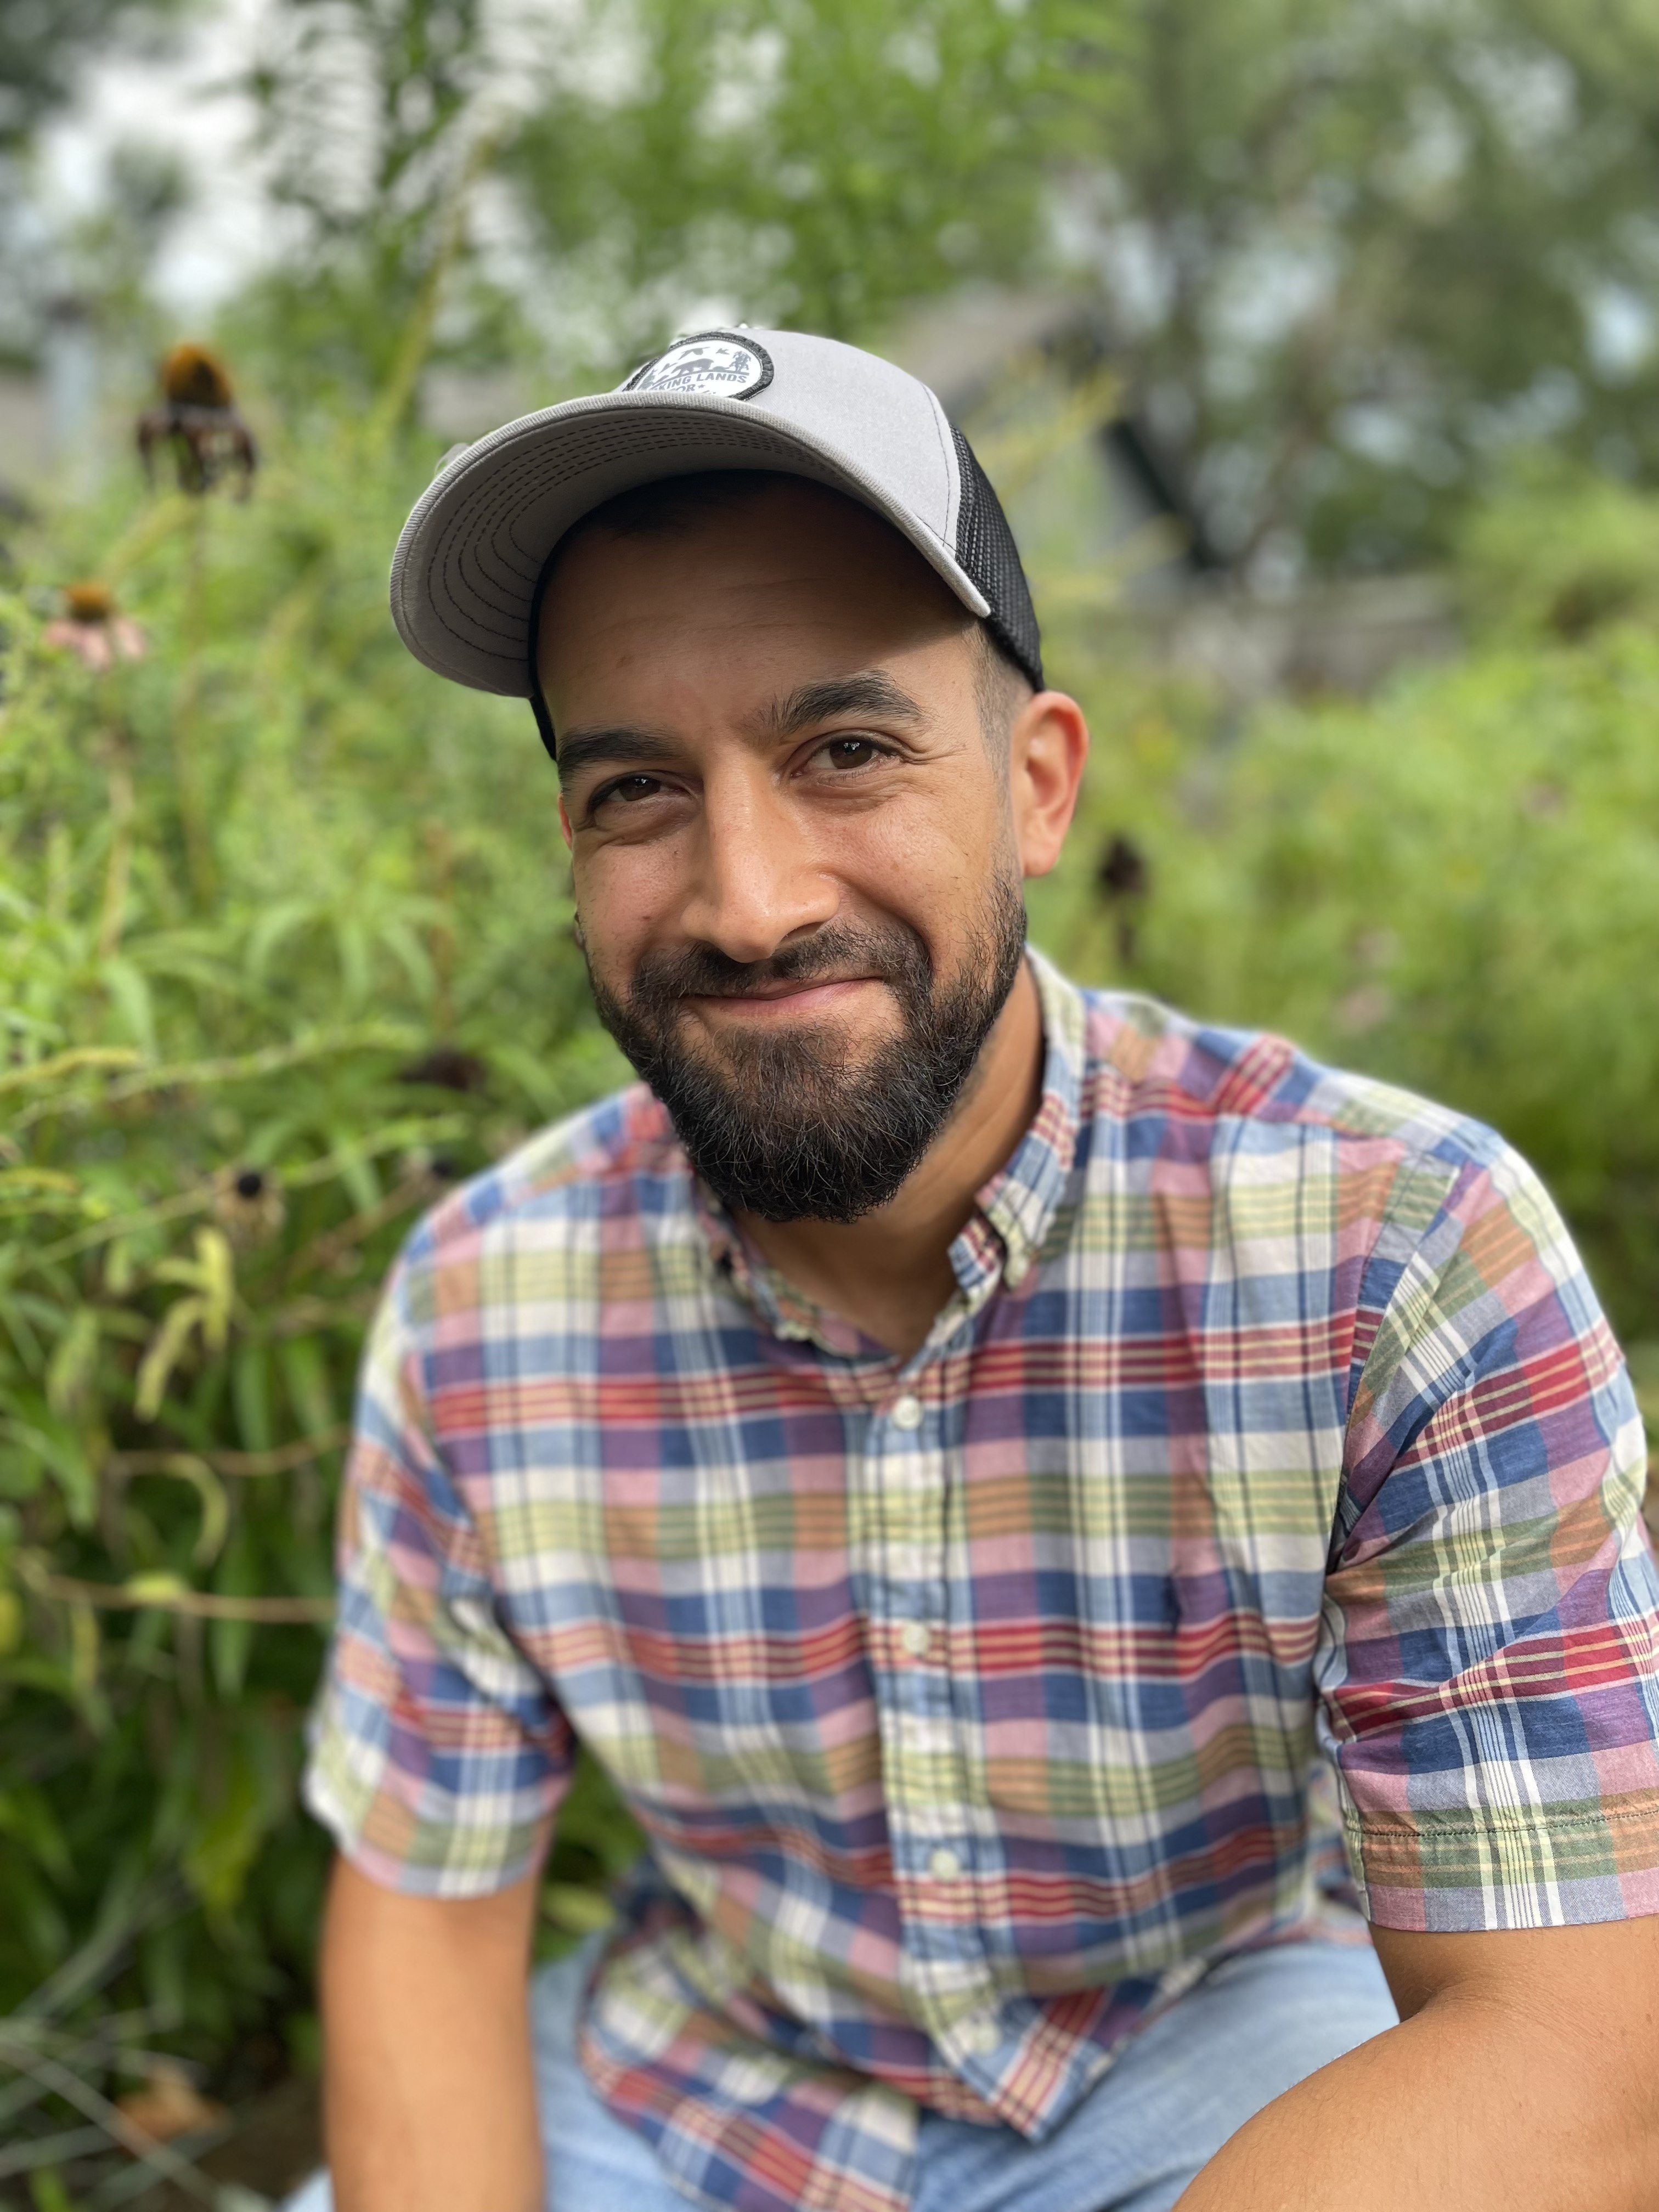
\includegraphics{C:/Users/Caleb/Box/GitHub/RobertsLabWebsite2/images/ProfilePics/ProfilePic_CalebRoberts.JPG}\\
\hline
\textbf{Jess Schmit} & Master's Student & jmschmit@uark.edu & Jess is incredibly excited to be joining the Living Landscapes Lab as a Masters’ student studying King Rails in Arkansas.  Her research interests are avian and wetland ecology, endangered species, habitat selection and resiliency in relation to climate change. Jess’ project will focus on King Rail breeding,  ecology, distribution and abundance in Arkansas, as well as their site selection and habitat use. She has been working as a wetland bird field technician for the last five years and has been blessed to work with a variety of species. Her last three years of work have been focused on rails, and she loves the challenge of working with these intelligent birds. Jess has a mailing address in Pennsylvania but is hardly home! When she isn’t in the field, she enjoys reading, kayaking, finding great local breakfast places wherever she lives, and hanging out with her husband and cat. & 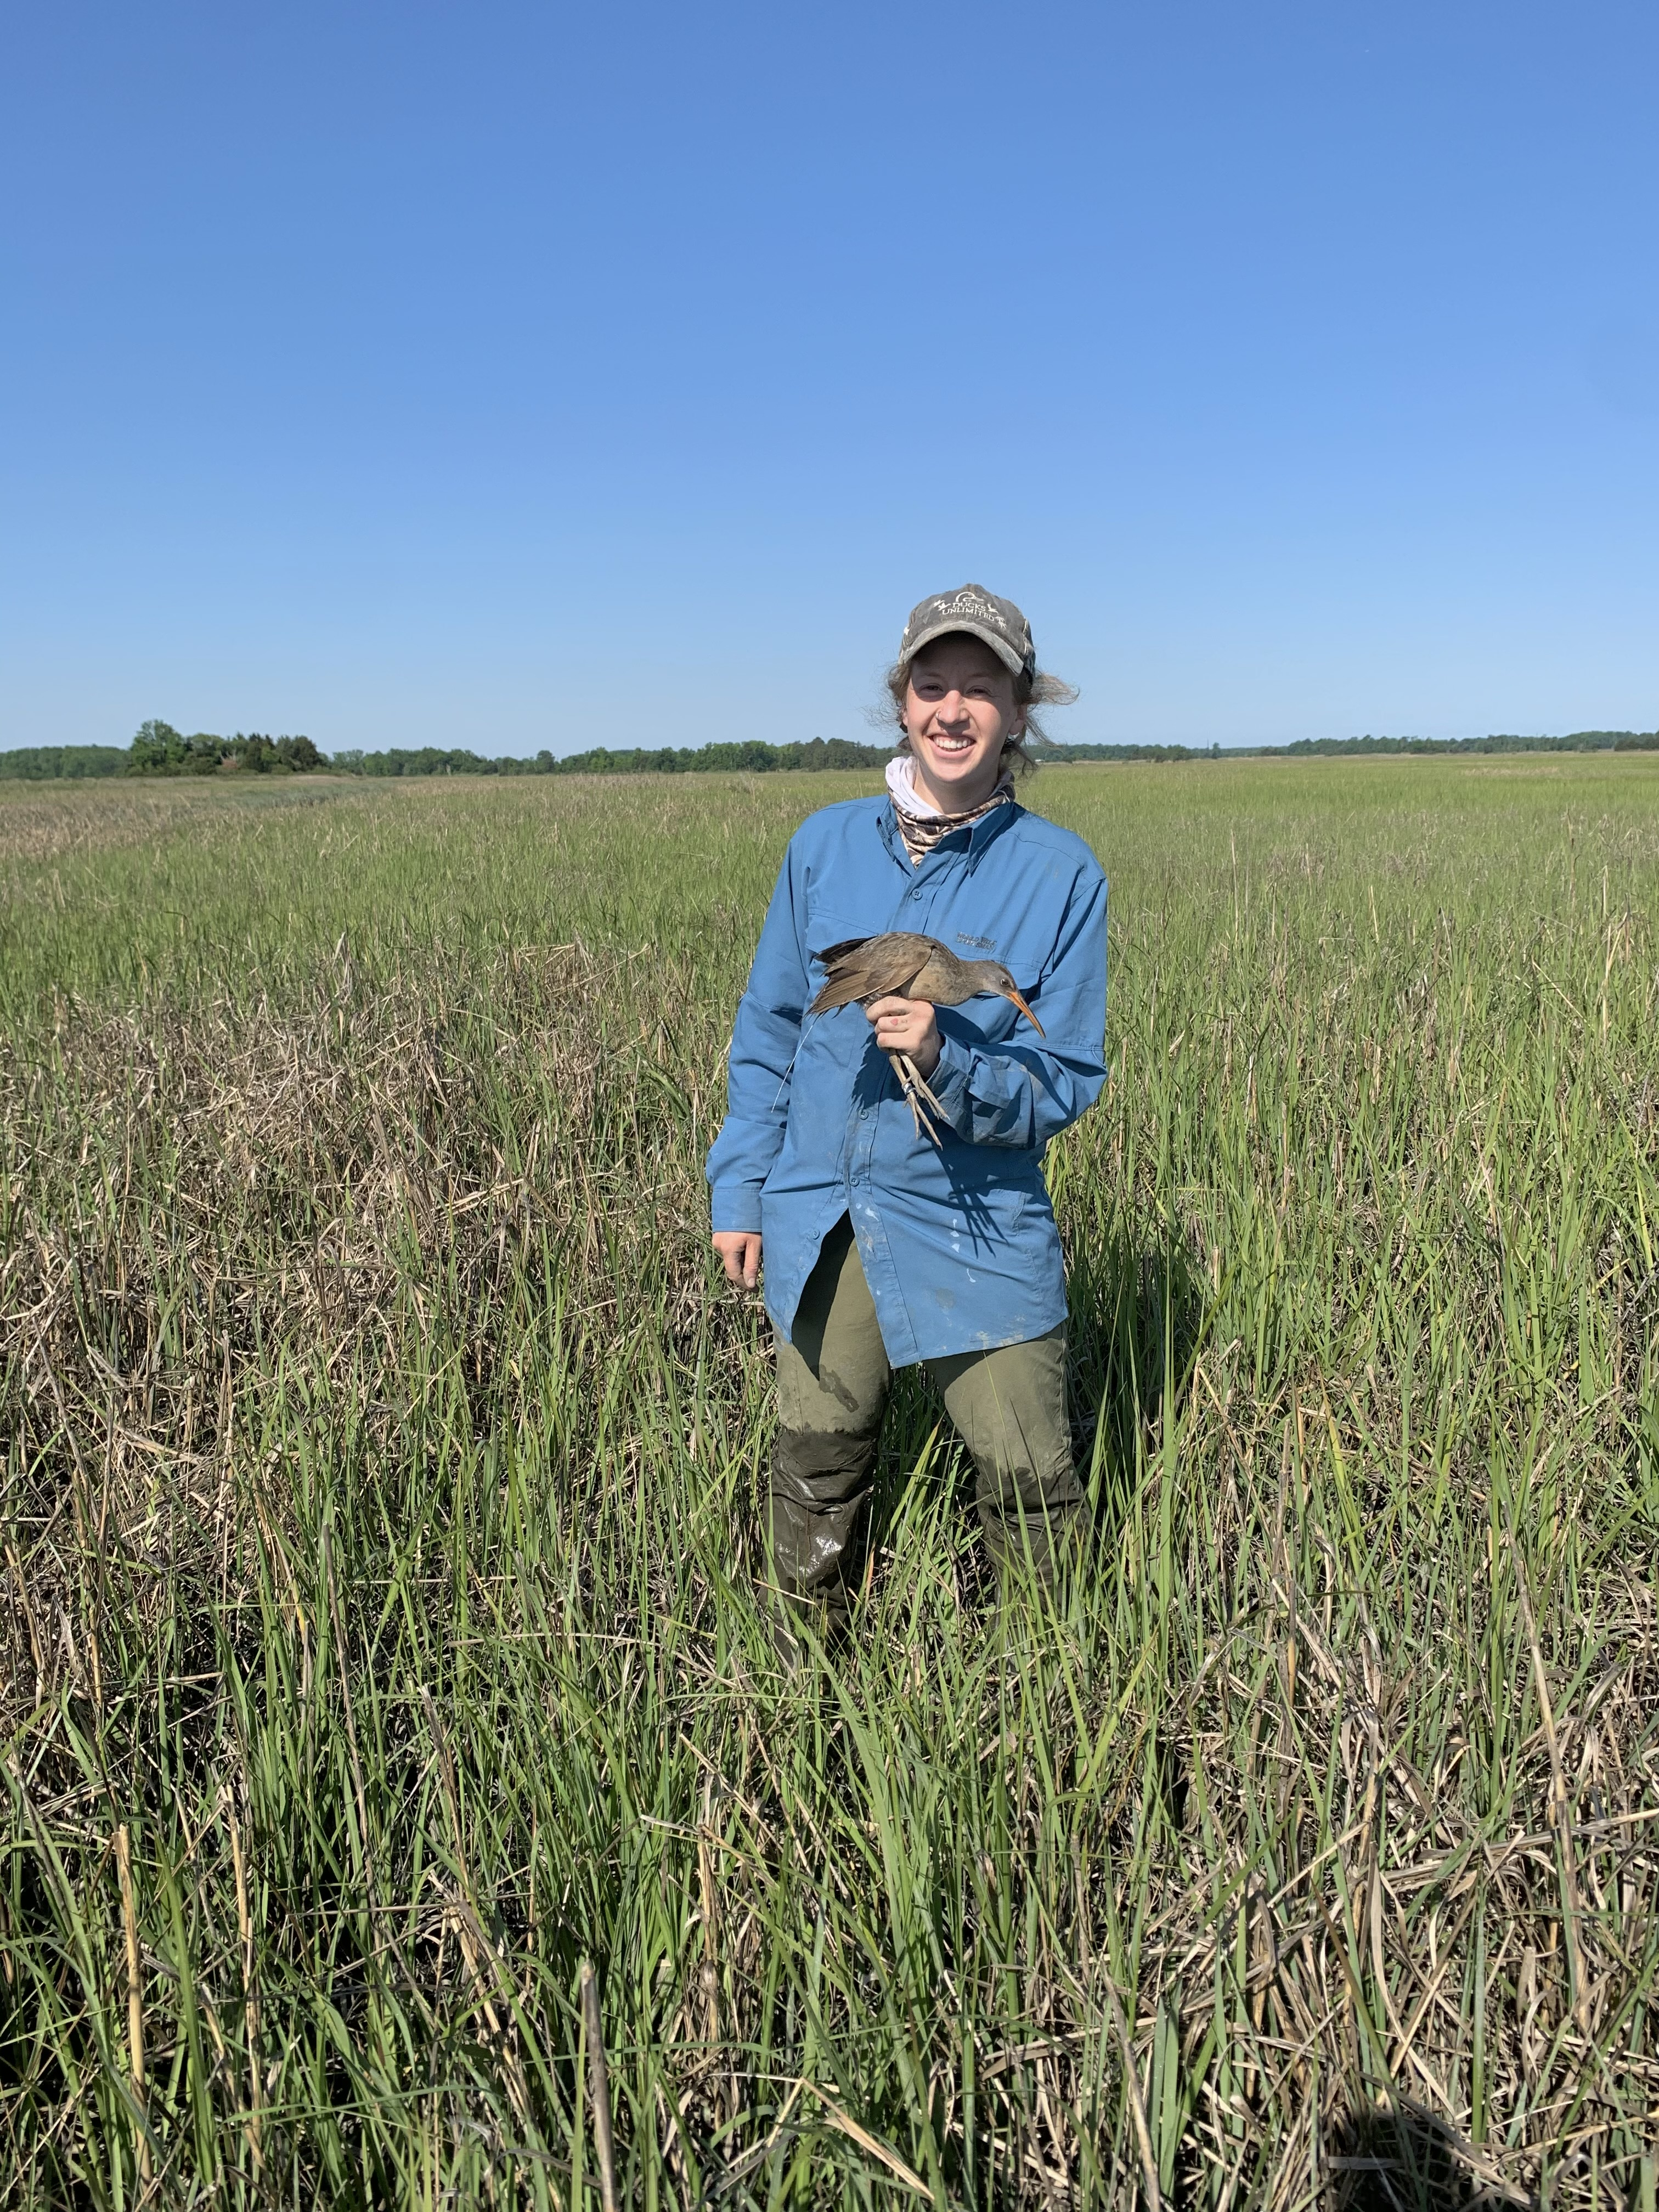
\includegraphics{C:/Users/Caleb/Box/GitHub/RobertsLabWebsite2/images/ProfilePics/ProfilePic_JessSchmit.jpg}\\
\hline
\textbf{Mike Shaw} & Master's Student & ms161@uark.edu & Mike’s research interests are in mammal ecology, and he will be studying Eastern Spotted Skunk (Spilogale putorius) in southwest Arkansas. He will be using camera traps to document the presence of Eastern spotted skunk and observe habitat associations. Mike worked in Colorado as a wildlife technician for Colorado Parks and Wildlife and moved to Maryland after his position in Colorado. In Maryland, he worked for county government as a wildlife management specialist. Mike is from eastern Maine, and he enjoys hiking, weightlifting, kayaking, and boardgames. & 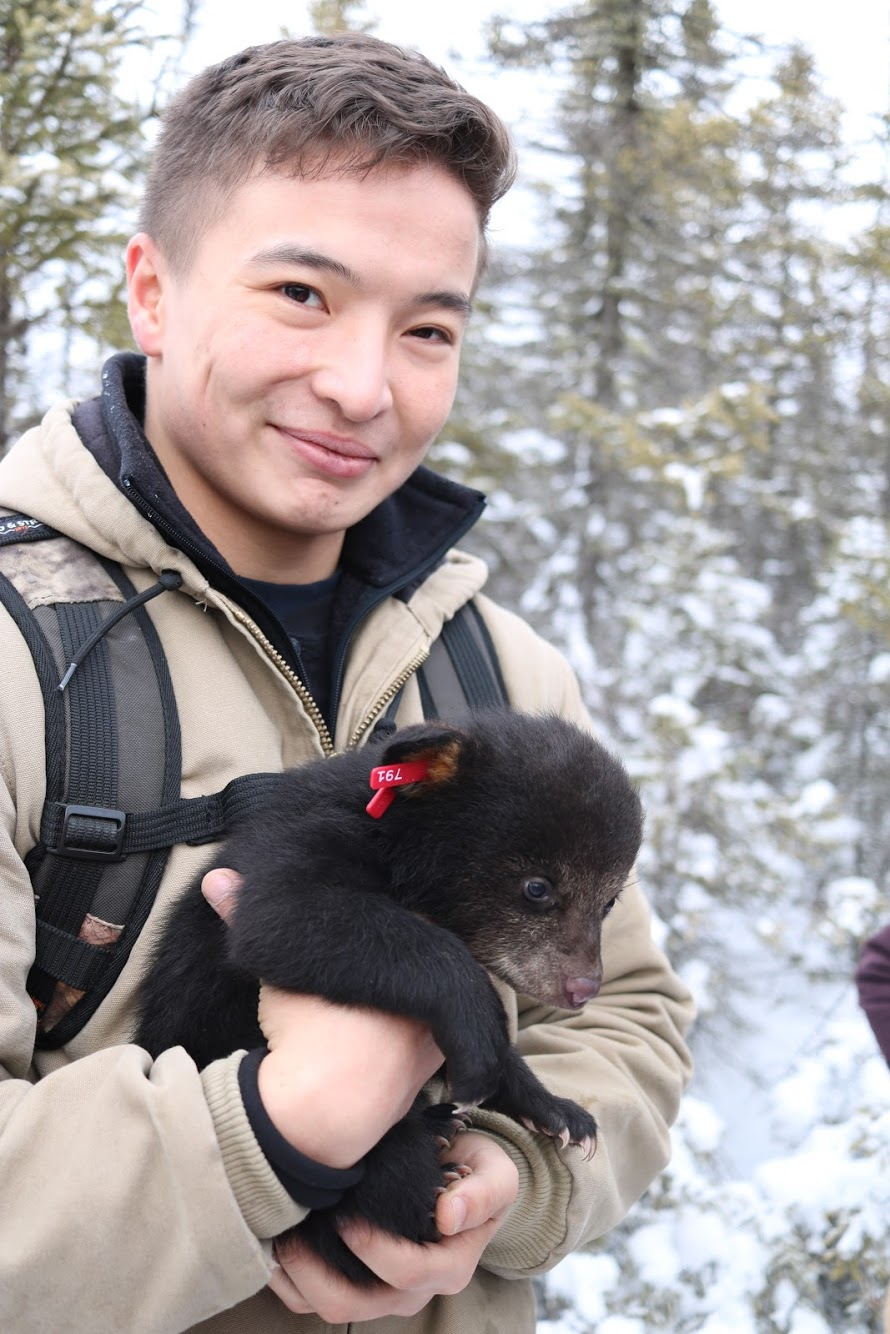
\includegraphics{C:/Users/Caleb/Box/GitHub/RobertsLabWebsite2/images/ProfilePics/ProfilePic_MichaelShaw.jpeg}\\
\hline
\textbf{Ken Wilson} & Master's Student & kw101@uark.edu & Ken’s research is focused on ground and shrub nesting birds in Southern Arkansas, and how they are impacted by the presence of feral hogs. Using camera traps, point count surveys, and vegetation surveys, Ken will measure the diversity and occupancy of breeding birds in bottomland hardwood floodplains and upland pine forests and how this is related to the density of feral hogs. This study will help us better understand how to manage a highly invasive species to protect vulnerable bird populations. Ken has previously worked for federal and state wildlife agencies studying secretive wetland birds, ground-nesting warblers, and pygmy owls, among other avian species. Ken is from New Jersey and in his free time, he enjoys reading, hiking, martial arts, and spending time with his cat. & 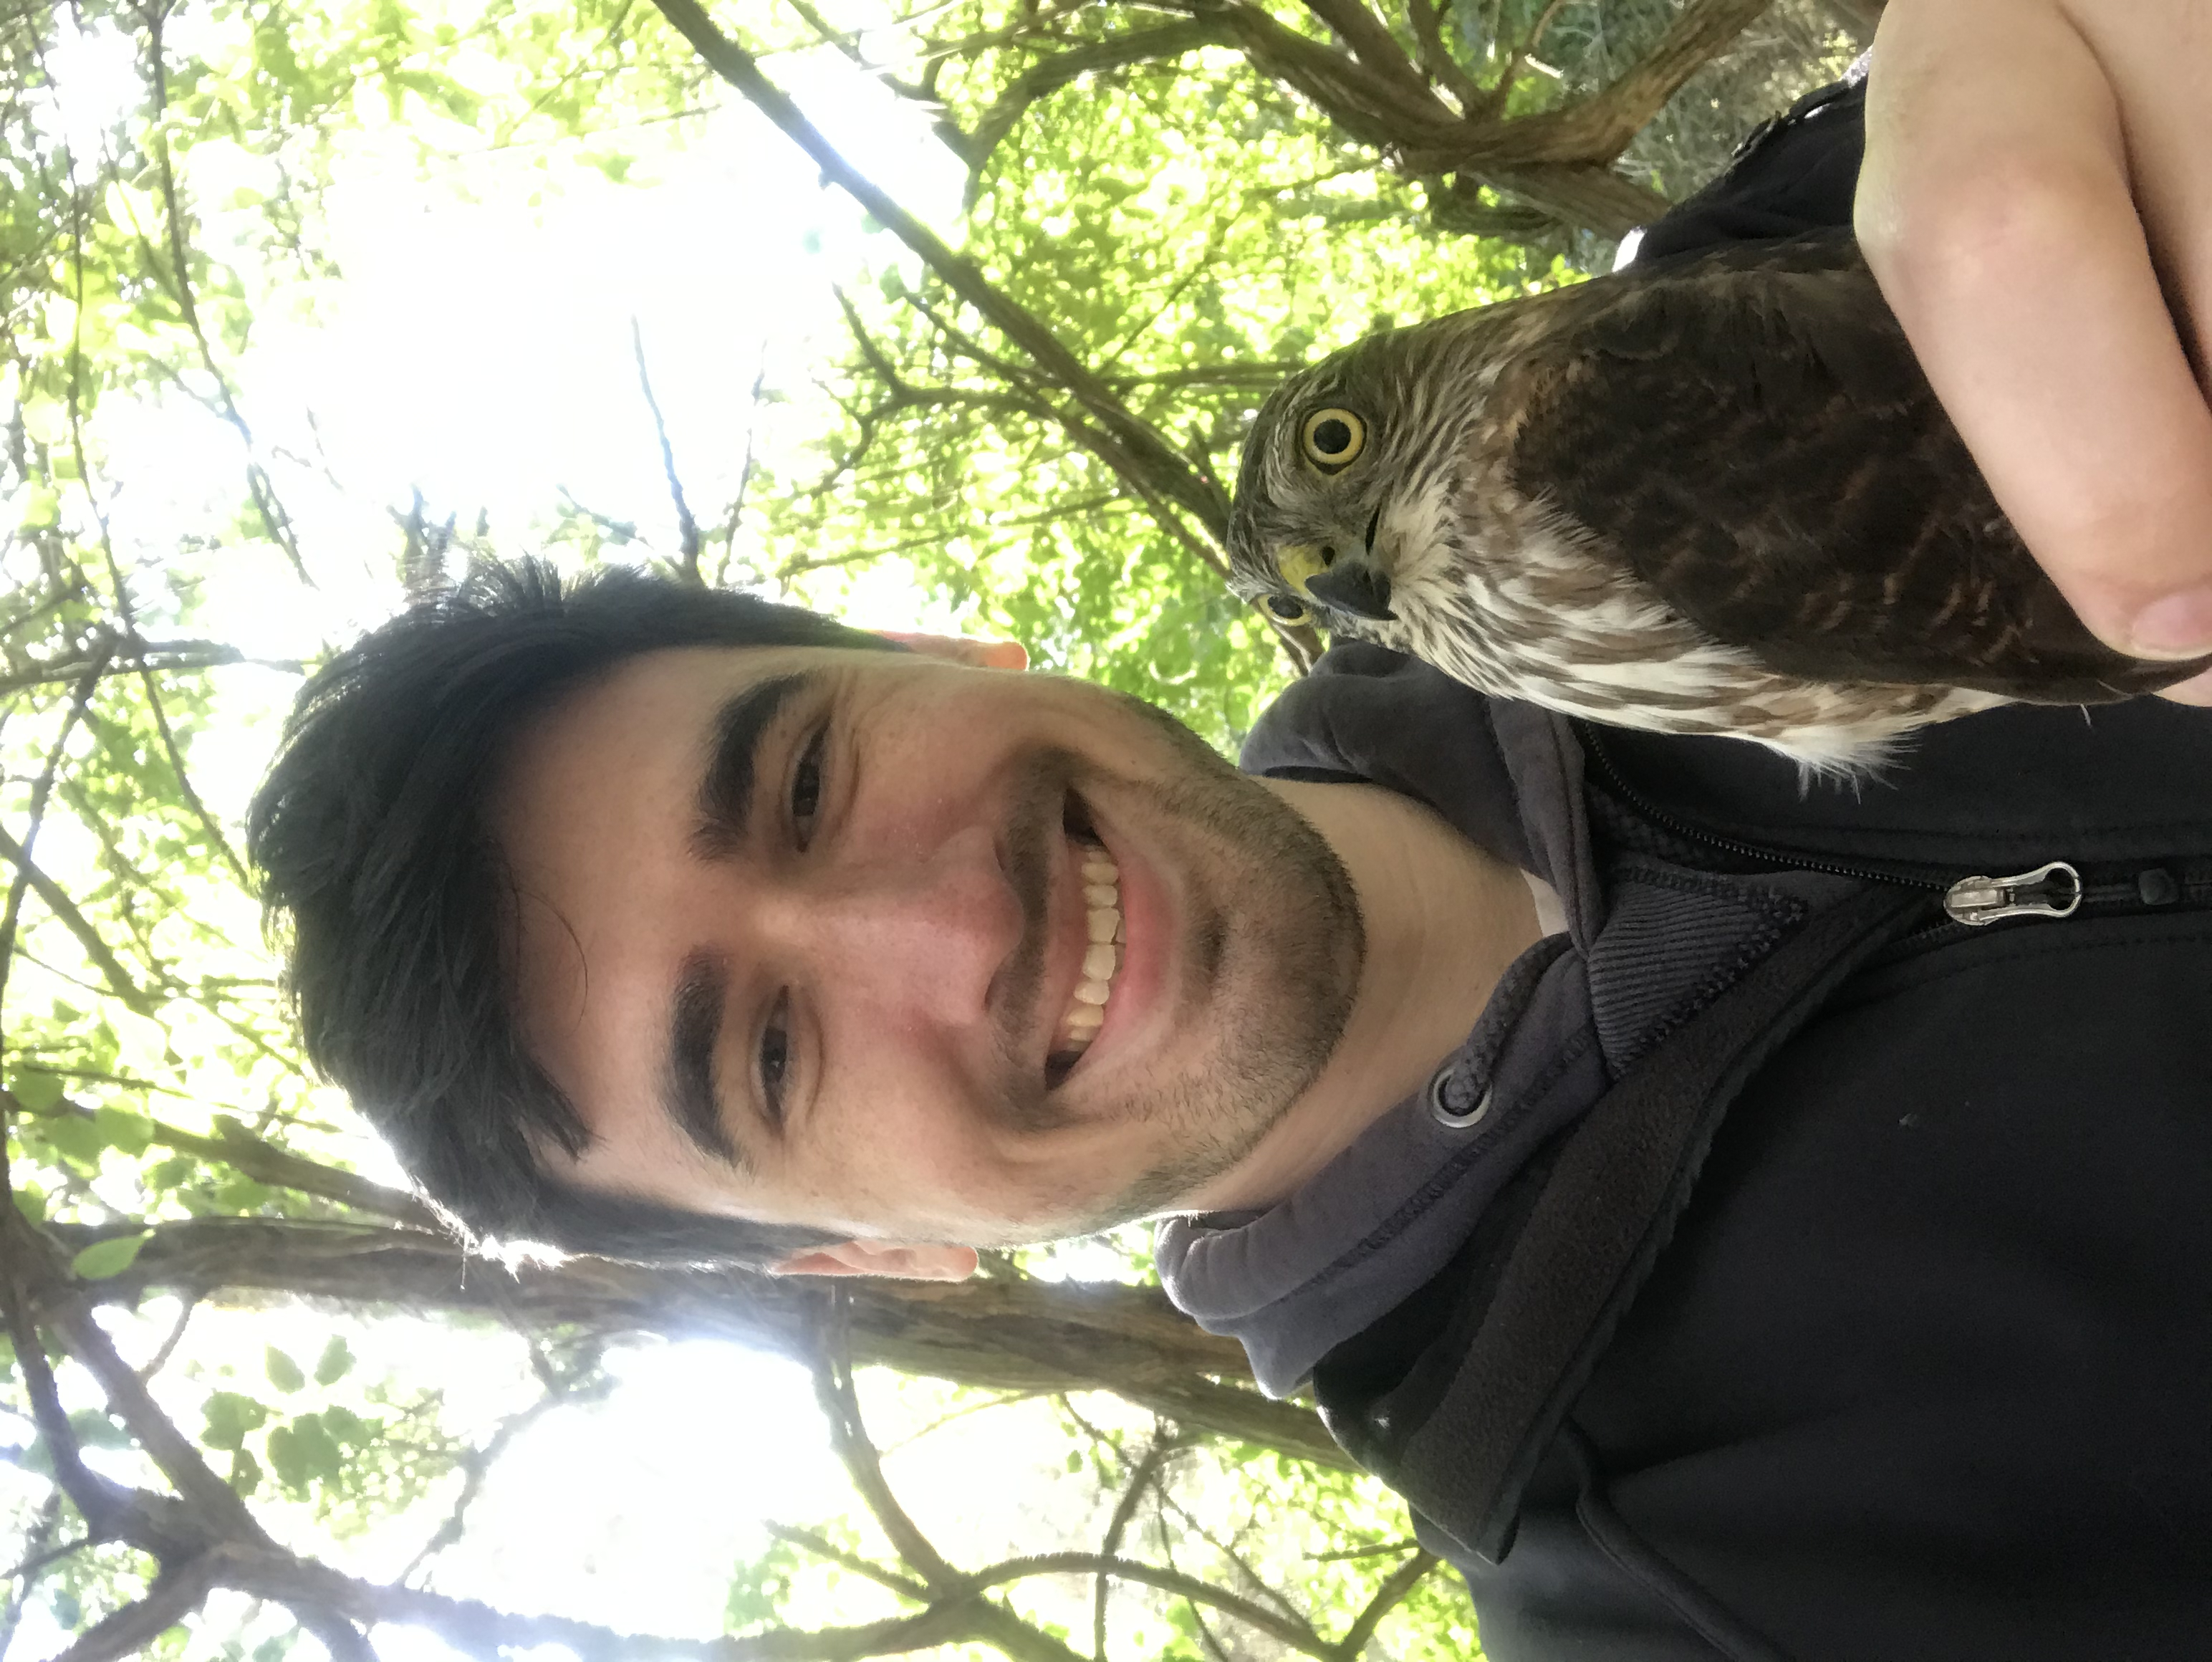
\includegraphics{C:/Users/Caleb/Box/GitHub/RobertsLabWebsite2/images/ProfilePics/ProfilePic_KenWilson.jpg}\\
\hline
\end{tabular}
\end{table}

\end{document}
